\documentclass{article}\usepackage[]{graphicx}\usepackage[]{color}
%% maxwidth is the original width if it is less than linewidth
%% otherwise use linewidth (to make sure the graphics do not exceed the margin)
\makeatletter
\def\maxwidth{ %
  \ifdim\Gin@nat@width>\linewidth
    \linewidth
  \else
    \Gin@nat@width
  \fi
}
\makeatother

\definecolor{fgcolor}{rgb}{0.345, 0.345, 0.345}
\newcommand{\hlnum}[1]{\textcolor[rgb]{0.686,0.059,0.569}{#1}}%
\newcommand{\hlstr}[1]{\textcolor[rgb]{0.192,0.494,0.8}{#1}}%
\newcommand{\hlcom}[1]{\textcolor[rgb]{0.678,0.584,0.686}{\textit{#1}}}%
\newcommand{\hlopt}[1]{\textcolor[rgb]{0,0,0}{#1}}%
\newcommand{\hlstd}[1]{\textcolor[rgb]{0.345,0.345,0.345}{#1}}%
\newcommand{\hlkwa}[1]{\textcolor[rgb]{0.161,0.373,0.58}{\textbf{#1}}}%
\newcommand{\hlkwb}[1]{\textcolor[rgb]{0.69,0.353,0.396}{#1}}%
\newcommand{\hlkwc}[1]{\textcolor[rgb]{0.333,0.667,0.333}{#1}}%
\newcommand{\hlkwd}[1]{\textcolor[rgb]{0.737,0.353,0.396}{\textbf{#1}}}%
\let\hlipl\hlkwb

\usepackage{framed}
\makeatletter
\newenvironment{kframe}{%
 \def\at@end@of@kframe{}%
 \ifinner\ifhmode%
  \def\at@end@of@kframe{\end{minipage}}%
  \begin{minipage}{\columnwidth}%
 \fi\fi%
 \def\FrameCommand##1{\hskip\@totalleftmargin \hskip-\fboxsep
 \colorbox{shadecolor}{##1}\hskip-\fboxsep
     % There is no \\@totalrightmargin, so:
     \hskip-\linewidth \hskip-\@totalleftmargin \hskip\columnwidth}%
 \MakeFramed {\advance\hsize-\width
   \@totalleftmargin\z@ \linewidth\hsize
   \@setminipage}}%
 {\par\unskip\endMakeFramed%
 \at@end@of@kframe}
\makeatother

\definecolor{shadecolor}{rgb}{.97, .97, .97}
\definecolor{messagecolor}{rgb}{0, 0, 0}
\definecolor{warningcolor}{rgb}{1, 0, 1}
\definecolor{errorcolor}{rgb}{1, 0, 0}
\newenvironment{knitrout}{}{} % an empty environment to be redefined in TeX

\usepackage{alltt}[12pt]
\usepackage{Sweave}
\usepackage{float}
\usepackage{graphicx}
\usepackage{tabularx}
\usepackage{siunitx}
\usepackage{amssymb} % for math symbols
\usepackage{amsmath} % for aligning equations
\usepackage{mdframed}
\usepackage{natbib}
\bibliographystyle{..//refs/styles/gcb}
\usepackage[hyphens]{url}
\usepackage[small]{caption}
\setlength{\captionmargin}{30pt}
\setlength{\abovecaptionskip}{0pt}
\setlength{\belowcaptionskip}{10pt}
\topmargin -1.5cm        
\oddsidemargin -0.04cm   
\evensidemargin -0.04cm
\textwidth 16.59cm
\textheight 21.94cm 
%\pagestyle{empty} %comment if want page numbers
\parskip 7.2pt
\renewcommand{\baselinestretch}{2}
\parindent 0pt
\usepackage{lineno}
\linenumbers
\usepackage{setspace}
\doublespacing

\newmdenv[
  topline=true,
  bottomline=true,
  skipabove=\topsep,
  skipbelow=\topsep
]{siderules}
\IfFileExists{upquote.sty}{\usepackage{upquote}}{}
\begin{document}
\noindent \textbf{\Large{Latitude Analysis Write-up}}
\section*{The effects of photoperiod across a species' latitudinal distribution}
The three major phenological cues that control spring budburst \citep[i.e., low winter temperatures, warm spring temperatures and increasing daylengths][]{Chuine2010} are important determinants of a species' range distribution. With recent warming temperatures, species distributions are predicted to shift poleward \citep{Chen2011, Chuine2001, Parmesan1999}, which would, in turn, affect the interaction of phenological cues an individual experiences. 

There is large debate over the role of photoperiod on budburst initiation across a species' latitudinal range. The predominating arguments are that (1) species from lower latitudes will be more reliant on photoperiod with climate change \citep{Zohner2016}, (2) photoperiod will slow or constrain range expansion \citep{Saikkonen2012}, (3) all species will rely on photoperiod more as winters warm \citep{Way2015}, and (4) lower latitude species will require both strong photoperiod cues and more forcing in order to compensate for the lack of chilling but photosensitivity may be more important at the cold trailing edge for range expansion to occur \citep{Gauzere2017}.

%\textit{Fagus sylvatica}, a well-documented species to be under strong photoperiodic control for budburst, is temperature limited at its northern distribution range \citep{Stromme2019}.

\section*{Methods for testing the effects of latitude on budburst}
To test for photoperiod sensitivity across latitudes, we designed a model that assesses the effects of each phenological cue on budburst in addition to the effect of latitude and we also included an interaction of photoperiod by latitude. Species were included if they were in multiple studies and if multiple cues were manipulated across studies. We also included species complexes in which species from the same genus would be included if they were represented across multiple studies and multiple cues were manipulated across those studies. We then subsetted the species and species complexes to include only those that had multiple provenance locations. 

We used a Bayesian mixed-effects hierarchical model approach to analyze our data to best estimate the day of budburst. We fit a guassian distribution model using forcing, chilling (i.e., measured as chill portions), photoperiod, latitude and the photoperiod by latitude two-way interaction as predictors (fixed effects) and species as modeled groups (random effects). The Bayesian model was fit using Stan modeling language \citep{Carpenter2017}(\texttt{www.mc-stan.org}), accessed via the \textit{rstan} package (version 2.15.1), version 2.3.1, in R \citep{R}, version 3.3.1, and was written as follows: 

\begin{align*}
y_i \thicksim N(\alpha_{sp[i]} +& \beta_{forcing_{sp[i]}} + \beta_{chilling_{sp[i]}} + \beta_{photoperiod_{sp[i]}} + \beta_{latitude_{sp[i]}}  \\
	+& \beta_{photoperiod x latitude_{sp[i]}} + \sigma_{sp_{(i)}}
\end{align*}

\noindent The $\alpha$ and each of the 5 $\beta$ coefficients were modeled at the species level, as follows:
\begin{align*}
1.& \; \beta_{forcing_{sp}} \thicksim N(\mu_{forcing}, \sigma{^2}_{forcing}) \\
   &... \\
5.& \; \beta_{photoperiod x latitude_{sp}} \thicksim N(\mu_{photoperiod x latitude}, \sigma{^2}_{photoperiod x latitude})
\end{align*}

We ran four chains, with 1,500 warm-up iterations followed by 2,500 sampling iterations, resulting in 10,000 posterior samples for each parameter. We assessed good model performance through $\hat{R}$ close to 1 and high $n_{eff}$ as well as visual consideration of chain convergence and posteriors \citep{Gelman2006}. 

\section*{Results for the effects of latitude on budburst}
Higher forcing tmeperatures, longer photoperiods, more chilling and higher latitudes advanced budburst, with more chilling having the largest effect (Figure \ref{fig:modelest}). Provenance latitude had the smallest effect on budburst (-2.89 days) and the greastest variation across species. Photoperiod and provenance latitude had a delayed interactive response, suggesting the two effects offset one another. As both higher latitudes and longer photoperiods advance the day of budburst, the interaction shows that the importance of photoperiod as a predictor decreases for sites that are at higher latitudes. Lower provenance latitudes were more responsive to higher photoperiod treatments (Figure \ref{fig:intrxn}). Higher provenance latitudes had earlier days of budburst, overall, and both high and low photoperiod treatments did not change budburst significantly. 

\section*{Main Takeaways}
\begin{enumerate}
\item Photoperiod plays a bigger role in determining day of budburst at lower latitudes.
\item Overall, individuals from higher latitudes initiated budburst slightly earlier, suggesting the phenological cue requirements are lower. 
\end{enumerate}


\bibliography{..//refs/latanalysis.bib}

{\begin{figure} [H]
  -\begin{center}
  -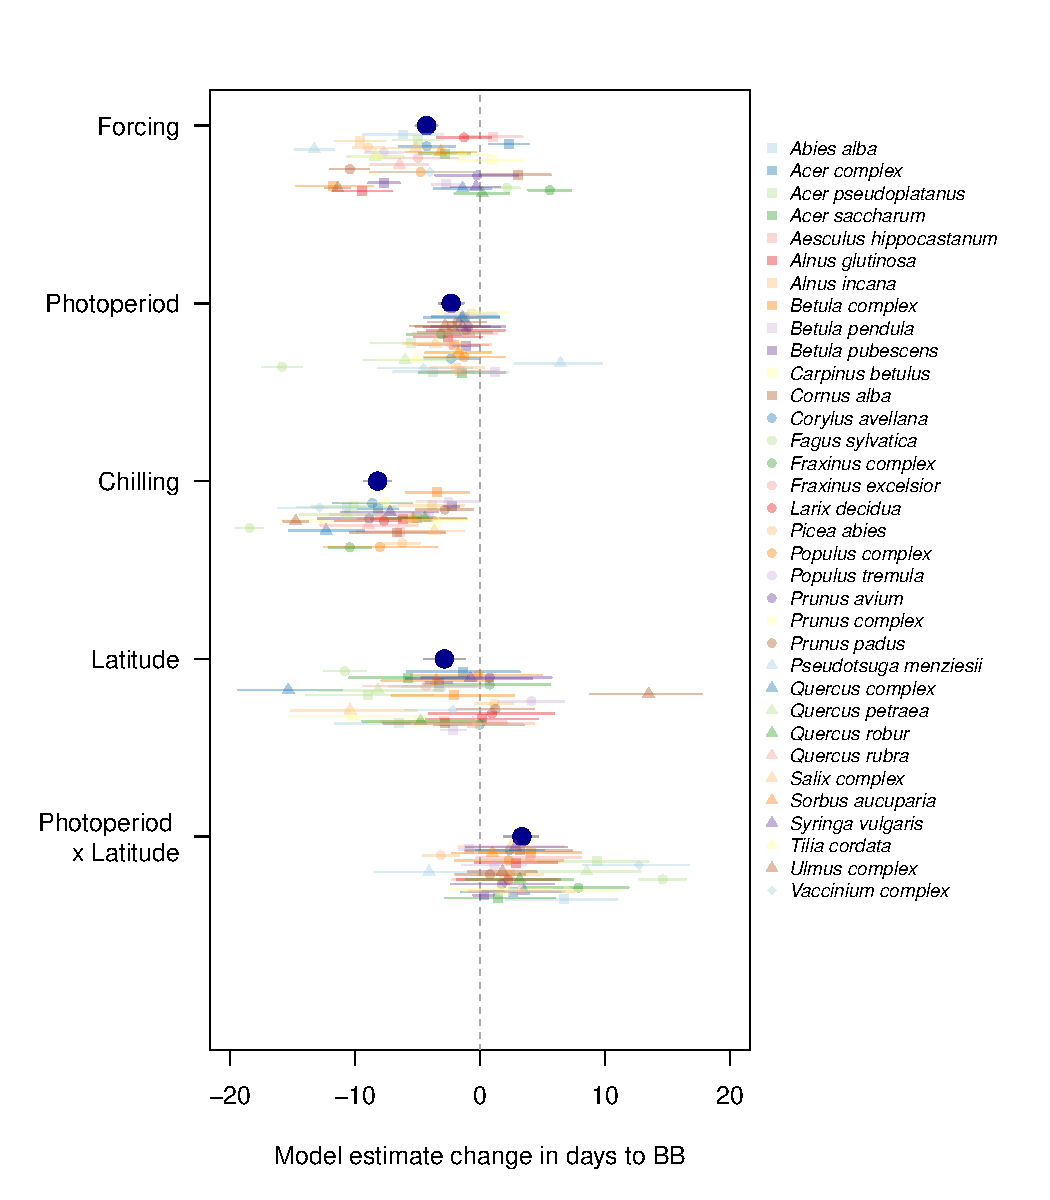
\includegraphics[width=14cm]{..//figures/latanalysis_spcom_expramp_fp.pdf}
  -\caption{The effects of forcing, photoperiod, chilling, latitude and latitude by photoperiod on day of budburst. The large, dark blue points and bars represent the mean and 50\% credible intervals and species-level vairations are shown in smaller points below the mean estimates. More positive values are delays in budburst, whereas more negative values are advances in budburst. As both higher latitudes and longer photoperiods advance the day of budburst, the interaction shows that the importance of photoperiod as a predictor decreases for sites that are at higher latitudes.  }\label{fig:modelest}
  -\end{center}
  -\end{figure}}

{\begin{figure} [H]
  -\begin{center}
  -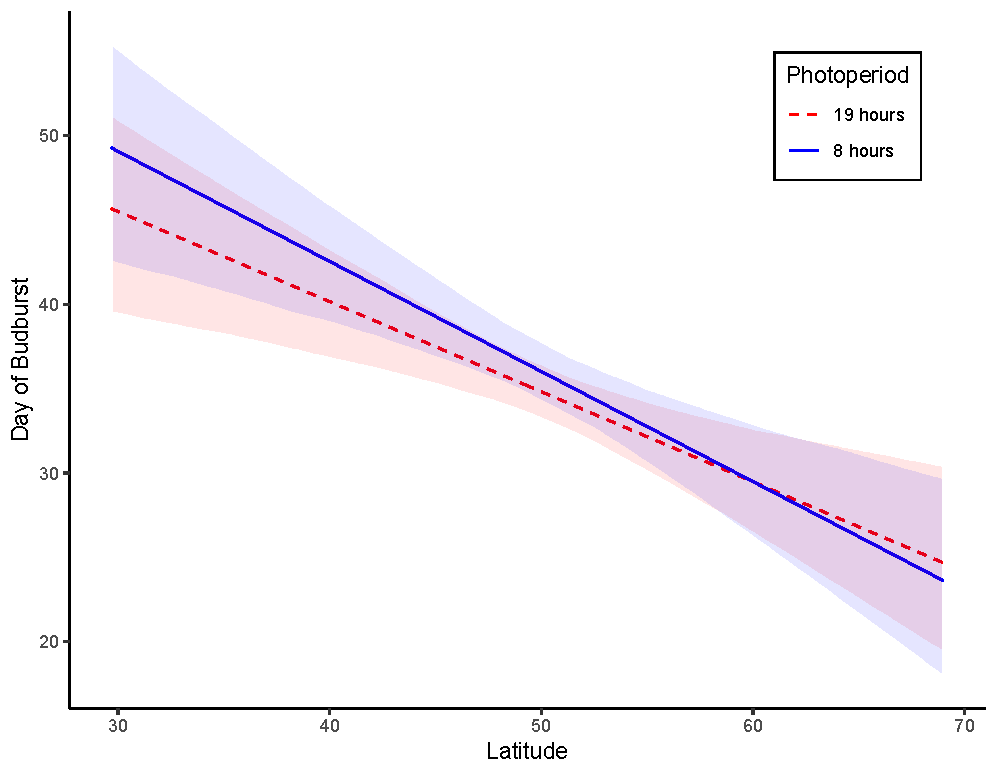
\includegraphics[width=10cm]{..//figures/LatxPhoto_allspp.pdf}
  -\caption{ The interactive effects of photoperiod and latitude on the day of budburst. With increasing provenance latitude, the day of budburst advances. Low photoperiod (8 hours) is the solid blue line and high photoperiod (19 hours) is the dashed red line. }\label{fig:intrxn}
  -\end{center}
  -\end{figure}}
  

\end{document}
